% Well ordering principle question
% Binary search correctness
% Mininum segment tree (recursive correctness)
% Runtime analysis
    % Prove that Big Theta is an equivalence relation (no)
    % Interpolation (no)
% Closed form for recursive functions (no)
% Master theorem
    % Definition
    % Tight asymptotic bound implies regularity
    % Application
% DFA
    % Interpret DFA for strings under length 3 or '100'
    % Create DFA for L((ab + a)*) and prove correctness
    % Prove that the language a^{n^2} is not regular
% Hellish loop correctness (idk yet)
    % Shortest length subarray that has a sum greater than or equal to M
\documentclass{article}
\usepackage{CJKutf8}
\usepackage{amsmath,amssymb,amsthm,enumerate,nicefrac,fancyhdr,hyperref,graphicx,adjustbox,mathtools}
\hypersetup{colorlinks=true,urlcolor=blue,citecolor=blue,linkcolor=blue}
\usepackage[left=3.5cm, right=3.5cm, top=1.5cm, includehead, includefoot]{geometry}
\usepackage[dvipsnames]{xcolor}
\usepackage[d]{esvect}
\usepackage{listings}
\usepackage{enumitem} % To allow for alph in enumerate
\usepackage[normalem]{ulem}
\usepackage{braket}
\usepackage{float} % To allow for H setting in figures.

% to draw dfas
\usepackage{tikz}
\usetikzlibrary{automata, positioning, arrows}

\begin{document}
    \tikzset{
        ->, % makes the edges directed
        >=stealth', % makes the arrow heads bold
        node distance=3cm, % specifies the minimum distance between two nodes. Change if necessary.
        every state/.style={thick, fill=gray!10}, % sets the properties for each ’state’ node
        initial text=$ $, % sets the text that appears on the start arrow
    }
    \lstset{
        numbers=left,
        mathescape=true,
        literate=
               {=}{$\leftarrow{}$}{1}
               {==}{$={}$}{1}
    }
    {\Large NAME (PRINT): \enspace\hrulefill}

    \bigskip

    {\Large STUDENT NUMBER (PRINT): \enspace\hrulefill}

    \bigskip

    \begin{center}
        \fbox{\parbox{\dimexpr\linewidth-2\fboxsep-2\fboxrule\relax}{
            \begin{center}
                \textbf{\Large University of Toronto Mississauga} \\

                \textbf{\Large FALL 2024 MOCK FINAL EXAMINATION} \\

                \textbf{\Large Introduction to Theory Computation} \\

                \textbf{\huge M\Large acho \huge M\Large an (m\^{}2)} \\

                \textbf{\Large Duration - \sout{3 hours} 10 minutes} \\

                \textbf{\Large Aids : \begin{CJK}{UTF8}{min}お前のお母さん\end{CJK}:} \\

                \textbf{\Large\url{https://youtu.be/3UHR_XWrGhc}}
            \end{center}

            \textit{\large The University of Toronto Mississauga and you, as a student, share a commitment to academic integrity. You are reminded that you may be charged with an academic offence for possessing any unauthorized aids during the writing of an exam. Clear, sealable, plastic bags have been provided for all electronic devices with storage, including but not limited to: cell phones, smart watches, SMART devices, tablets, laptops, and calculators. Please turn off all devices, seal them in the bag provided, and place the bag under your desk for the duration of the examination. You will not be able to touch the bag or its contents until the exam is over.}

            \medskip

            \textit{\large If, during an exam, any of these items are found on your person or in the area of your desk other than in the clear, sealable, plastic bag, you may be charged with an academic offence. A typical penalty for an academic offence may cause you to fail the course.}

            \medskip

            \textit{\large Please note, once this exam has begun, you \textbf{CANNOT} re-write it.}
        }}
    \end{center}

    \noindent This is a mock exam designed for studying CSC236. Any and all similarities with the Fall 2024 CSC236 final examination are purely coincidence.

    \noindent This examination is meant to be done in 3 hours, but it is a little bit long, so do not worry about finishing. Part marks are very easy to get! :))))))))))))) There are a total of 9 questions worth a total of 78 points. Answer the questions in the space provided. If you require extra space for a question, use the extra pages at the end of the exam and clearly label on the said question's page that you are using the extra pages.

    \pagebreak

    \noindent\textbf{Q1. (9 points)} Consider the DFA below:
    \begin{center}
        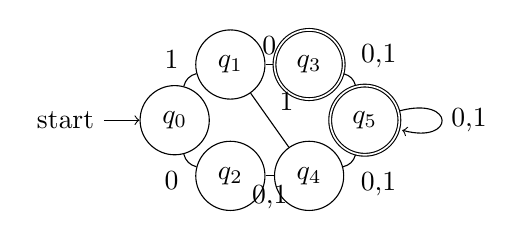
\begin{tikzpicture}
            \node[state, initial] (q0) {\(q_0\)};
            \node[state, above right of=q0] (q1) {\(q_1\)};
            \node[state, below right of=q0] (q2) {\(q_2\)};
            \node[state, accepting, right of=q1] (q3) {\(q_3\)};
            \node[state, right of=q2] (q4) {\(q_4\)};
            \node[state, accepting, below right of=q3] (q5) {\(q_5\)};

            \draw (q0) edge[bend left, above left] node{1} (q1)
                  (q0) edge[bend right, below left] node{0} (q2)
                  (q1) edge[above] node{0} (q3)
                  (q1) edge[above right] node{1} (q4)
                  (q2) edge[below] node{0,1} (q4)
                  (q3) edge[bend left, above right] node{0,1} (q5)
                  (q4) edge[bend right, below right] node{0,1} (q5)
                  (q5) edge[loop right] node{0,1} (q5);
        \end{tikzpicture}
    \end{center}
    \begin{enumerate}[label=\alph*)]
        \item (1 point) Describe the language accepted by the following DFA.

        \item (3 points) Convert this DFA into a minimal NFA (i.e., there is no smaller NFA that accepts this language). Give a brief justification for why it works.
        
        \pagebreak

        \item  (2 points) Provide a DFA that accepts the language matched by \((a+ab)^*\), where \(\Sigma = \{a, b\}\).
        \vfill
        \item (3 points) Prove the correctness of the DFA you provided.
        \vfill
    \end{enumerate}

    \pagebreak

    \noindent\textbf{Q2. (10 points)} For each of the statements below, decide whether it is \textbf{true or false} and provide a proof justifying your answer.

    \begin{enumerate}[label=\alph*)]
        \item (2 points) Let \(\Sigma = \{0, 1\}\). The language \(L = \{w \in \Sigma ^* : |w| = 3\}\) is regular.
        \vfill
        \item (2 points) Let \(\Sigma = \{0, 1\}\). \(L = \{1^{i}0^j : i,j \in \mathbb{N}, i \geq j\}\) is a regular language.
        \vfill
        \item (2 points) Let \(L, M\) be regular languages. The language \(L \cap M\) is regular.
        \vfill
        \pagebreak
        \item (2 points) Let \(\Sigma = \{a, b, c\}\). The language of all strings whose characters are alphabetically ordered is regular.
        \vfill
        \item (2 points) Let \(L, M\) be languages. If \(L\) is not regular, then \(L \cup M\) is not regular.
        \vfill
    \end{enumerate}

    \pagebreak

    \noindent\textbf{Q3. (6 points)}
    \begin{enumerate}[label=\alph*)]
        \item (2 points) State the CLRS version of master theorem. Define all variables and state their conditions.
        \vfill
        \item (4 points) Let \(f: \mathbb{N} \to \mathbb{R}\) be a nonnegative function. Prove that if \(f \in \Theta (n^k)\) for some \(k > 0\), then the regularity condition holds true.
        \vfill
    \end{enumerate}

    \pagebreak

    \noindent\textbf{Q4. (7 points)} Consider the program below:
    \begin{lstlisting}[language=Python]
    def binary_search(x: int, lst: list[int]):
        l = 0, r = len(lst) - 1
        while(r - l > 0):
            mid = (l+r) // 2
            if(lst[mid] == x):
                return mid
            elif(lst[mid] < x):
                r = mid
            else:
                l = mid + 1
        if(lst[l] == x):
            return l
        return -1
    \end{lstlisting}
    \begin{enumerate}[label=\alph*)]
        \item (2 points) State the preconditions and postconditions of this program.
        \item (5 points) Prove that this program is correct.
    \end{enumerate}
    
    \pagebreak

    \noindent\textbf{Q5. (6 points)} Let \(A\) be a set of functions defined recursively as follows:
    \begin{itemize}
        \item \(\sqrt{x} \in A\) 
        \item If \(f \in A\), then \(\frac{1}{f} - f \in A\) 
    \end{itemize}
    
    \begin{enumerate}[label=\alph*)]
        \item (4 points) Let \(P(f)\) be a predicate on \(A\) and suppose you have managed to prove that
        \begin{itemize}
            \item \(P(\sqrt{x})\) is true,
            \item \(P(f) \implies P(\frac{1}{f} - f)\) for all \(f \in A\).
        \end{itemize}
        Prove that \(\forall f \in A, P(f)\). You may only assume that the principle of induction holds for the natural numbers, NOT the set \(A\).
        \vfill
        \item (2 points) Prove that \(\forall f \in A\), \(f \left( \frac{1}{2} \right) = \frac{1}{\sqrt{2}}\).
        \vfill
    \end{enumerate}

    \pagebreak

    \noindent\textbf{Q6. (7 points)} Let \(\Sigma = \{0, 1\}\). For any language \(L \in \Sigma ^*\), define
    \[
        S = \{w \in \Sigma ^* : 0w1 \in L\}
    \]
    Given that \(L\) is a regular language, prove that \(S\) is a regular language.

    \pagebreak

    Now, this is where a normal exam would end. However, this is not a normal exam.

    \bigskip

    \noindent\textbf{Q7. (8 points)} Recall that a segment tree is a data structure effective for querying and updating information about a range of values in a list, such as the minimum element in a provided range. In fact, we will examine an implementation of a segment tree that does this.

    \medskip

    Suppose that we have a list of numbers \texttt{lst}. In this implementation, the segment tree can be thought of as a binary tree, with each node storing a range of indices \texttt{[l, r]}, a value which represents the minimum number in \texttt{lst[l:r]} (inclusive of both sides), and pointers to a left and right child. \textbf{Note that a node does not have a left and right child if and only if it is true that} \texttt{l = r}. Otherwise, the left child will keep track of the range \texttt{[l, \(\left\lfloor \frac{\texttt{l + r}}{2} \right\rfloor\)]} and the right child will track \texttt{[\(\left\lfloor \frac{\texttt{l + r}}{2} \right\rfloor\) + 1, r]}

    \medskip

    As an example, consider the following pseudocode for \texttt{update}, which updates the segment tree to correctly return queries about \texttt{lst} after setting \texttt{lst[i] = x}:

    \begin{lstlisting}[language=Python]
        def update(root: Node, x: int, i: int):
            if i not in [root.l, root.r] then return
            else if root.l == i == root.r then
                root.val = x
                return
            update(root.left_child, x, i)
            update(root.right_child, x, i)
            root.val = min(root.left_child.val, root.right_child.val)
    \end{lstlisting}
    \begin{enumerate}[label=\alph*)]
        \item (3 points) Prove that this method is correct.
        \pagebreak
        \item (3 points) Find the recursive worst-case runtime of \texttt{update}.
        \vfill
        \item (2 points) Find the tight asymptotic bound for the runtime of \texttt{update}.
        \vfill
    \end{enumerate}

    \pagebreak

    \textbf{Q8. (15 points)} Recall the statement of the \textit{pumping lemma:}

    \smallskip

    \noindent Let \(L\) be a regular language associated with some alphabet \(\Sigma\). Then \(\exists p \in \mathbb{N} ^+, \forall w \in L\), where \(|w| \geq p\), \(\exists x,y,z \in \Sigma ^*\) so that
    \begin{itemize}
        \item \(|y| \geq 1\)
        \item \(|xy| \leq p\)
        \item \(\forall n \in \mathbb{N}, xy^nz \in L\) 
    \end{itemize}

    \begin{enumerate}[label=\alph*)]
        \item (3 points) Show why the statement must have the condition \(|xy| \leq p\). (Hint: Consider the language \(\{w \in \{a, b\}^* : w = a^i b^j , i \leq j\}\))
        \vfill
        \item (2 points) Find with proof the value of \(p\) for the language \(\mathcal{L}(((ab)^*a)^*)\) 
        \vfill
        \item (1 point) Explain why every finite language can be pumped.
        \vfill
        \pagebreak
        Now, assume that \(L,M\) are regular languages that satisfy the pumping lemma, that is, they each have a value \(p_L\) and \(p_M\) that make the statement of the pumping lemma true. We say that a language can be \textbf{pumped} if it satisfies this property.
        
        \item (2 points) Prove that \(L \cup M\) can also be pumped.
        \vfill
        \item (2 points) Prove that \(M^*\) can be pumped (You would want to consider when \(M\) is finite or when \(M\) is infinite).
        \vfill
        \pagebreak
        \item (3 points) Prove that \(LM\) can be pumped.
        \vfill
        \item (2 points) Prove the pumping lemma.
        \vfill
    \end{enumerate}

    \pagebreak

    \textbf{Q9. (10 points)} Given two bits of either 0 or 1, the XOR operator returns 1 if and only if exactly one of the bits is 1. This operator can be generalised to be used with binary strings by comparing each individual bit. It is denoted by the symbol \^{}. When given integer inputs, the operator will automaticall convert them to binary, perform the operation, and output the result as a decimal number. This operator can be quite useful, as it will be illustrated in this question.

    Consider a list with with the property that there is only one number whose number of occurences in the list is odd. You can also think of it as every number having an even number of occurences except for one number. Take a look at the method below:

    \begin{lstlisting}[language=Python]
        def find_odd_number(A):
            '''
            Pre: A is a list with x being the only number having an
            odd number of occurences
            Post: Returns the odd element x
            '''
            m = 0
            i = 0
            while i < len(lst):
                m = m^lst[i]
                i = i + 1
            return m
    \end{lstlisting}

    \noindent Prove the correctness of this program. You may use the fact that the XOR operator is commutative.
    \vfill
    \newpage
    Extra page 1
    \newpage
    Extra page 2
\end{document}